% !TEX root = ../../main.tex

% Reset graphics to the current folder
\graphicspath{ {\thisch/figures/} }

\chapter{Appendix for \autoref{dut}}%
\label{appx:dut}

\section{Table of properties for low temperature probes}%
\label{appx:dut:probes}

\begin{table}[htbp]
	\centering\small
    \caption{Properties of probe gasses used at \SI{77}{\kelvin}.}
	\begin{tabular}{lccccc}
		\toprule
	    \textbf{Probe}
        & \textbf{Shape}
        & \textbf{Liquid density}
        & \textbf{Solid density}
        & \textbf{Dipole moment}
        & \textbf{Quadrupole moment} \\
        & & \si{\gram\per\metre^3} & \si{\gram\per\metre^3} & ESU & Debye \\
		\midrule
        \ce{Ar} & spherical & 28 & 27 & x & y \\
        \ce{CO} & linear    & 28 & 27 & x & y \\
        \ce{N2} & linear    & 28 & 27 & x & y \\
        \ce{O2} & linear    & 28 & 27 & x & y \\
        \bottomrule
	\end{tabular}%
	\label{appx:dut:tab:rtc-exp}
\end{table}%


\section{List of all experiments performed}

\begin{table}[htbp]
	\centering\small
    \caption{Summary of ambient temperature calorimetry experiments
    performed at \SI{77}{\kelvin}. Probe used is butane unless 
    explicitly stated.}
	\begin{tabular}{lll}
		\toprule
	    \textbf{Material}
        & \textbf{Conditions}
        & \textbf{Observations} \\
        \multicolumn{3}{c}{\scriptsize{\textit{C = cell, E = experiment, m = mass (mg)}}}\\
		\midrule
        DUT-46    & C1, E1, \(m\approx35\) & non-flexible \\
        DUT-46    & C1, E2 & non-flexible \\
        DUT-48    & C1, E1, \(m\approx10\)  & non-flexible \\
        DUT-48    & C1, E2 & non-flexible \\
        DUT-48    & \textbf{\ce{C3H8}}, C1, E3 & no observed interactions \\
        DUT-48    & \textbf{\ce{C3H6}}, C1, E4 & increased enthalpy at low loading \\
        DUT-48    & \textbf{\ce{CO}}, C1, E5 & no observed interactions \\
        DUT-49(o) & C1, E1, \(m\approx97\)  & NGA \\
        DUT-49(o) & C1, E2  & sample decomposed \\
        DUT-49(m) & C2, E1, \(m\approx42\)  & NGA \\
        DUT-49(m) & C3, E1, \(m\approx38\)  & NGA \\
        DUT-49(m) & C4, E1, \(m\approx18\)  & NGA \\
        DUT-50    & C1, E1, \(m\approx24\)  & NGA \\
        DUT-50    & C1, E2 & sample decomposed \\
        DUT-50    & C2, E1, \(m\approx6\)  & NGA \\
        DUT-147   & C1, E1, \(m\approx18\)  & non-flexible \\
        DUT-148   & C1, E1, \(m\approx10\)  & NGA \\
        DUT-149   & C1, E1, \(m\approx45\)  & non-flexible \\
        DUT-149   & C1, E2, \(m\approx45\)  & non-flexible \\
        DUT-151   & C1, E1, \(m\approx15\)  & complex transitions \\
        DUT-151   & C1, E2 & complex transitions \\
        DUT-152   & C1, E1, \(m\approx30\)  & complex transitions \\
        DUT-160   & C1, E1, \(m\approx22\)  & NGA \\
        DUT-170   & C1, E1, \(m\approx23\)  & non-flexible, low sensitivity \\
        DUT-170   & C1, E2 & non-flexible \\
        DUT-171   & C1, E1, \(m\approx35\)  & continuous transition \\
        \bottomrule
	\end{tabular}%
	\label{appx:dut:tab:rtc-exp}
\end{table}%

\begin{table}[htbp]
	\centering\small
    \caption{Summary of low temperature calorimetry experiments. Conditions
    are identical for subsequent experiments unless explicitly stated.}
	\begin{tabular}{lcll}
		\toprule
	    \textbf{Material}
        & \textbf{Probe} 
        & \textbf{Conditions}
        & \textbf{Observations} \\
        \multicolumn{4}{c}{\scriptsize{\textit{C = cell, E = experiment, HF/LF = high/low flowrate, m = mass (mg)}}}\\
		\midrule
        DUT-49(o)  & \ce{Ar}   & C1, E1, LF, \(m\approx180\) & NGA \\
        DUT-49(o)  & \ce{Ar}   & C2, E1, LF, \(m\approx20\)  & NGA \\
        DUT-49(o)  & \ce{O2}   & C3, E1, LF, \(m\approx20\)  & NGA \\
        DUT-49(o)  & \ce{N2}   & C4, E1, LF, \(m\approx10\)  & NGA, additional transitions \\
        DUT-49(o)  & \ce{N2}   & C5, E1, LF, \(m\approx5\)   & NGA, additional transitions \\
        DUT-49(o)  & \ce{N2}   & C5, E2, LF & no NGA, additional transitions \\
        DUT-49(o)  & \ce{N2}   & C5, E3, LF & no NGA, additional transitions\\
        DUT-49(o)  & \ce{O2}   & C5, E4, LF & NGA \\

        DUT-49(m)  & \ce{CO}   & C6, E1, HF, \(m\approx20\)  & no NGA \\
        DUT-49(m)  & \ce{N2}   & C6, E2, HF & NGA, additional transitions \\
        DUT-49(m)  & \ce{CO}   & C7, E1, HF, \(m\approx20\)  & no NGA \\
        DUT-49(m)  & \ce{Ar}   & C7, E2, HF & NGA \\

        DUT-149    & \ce{N2}   & C1, E1, LF, \(m\approx10\)  & no NGA \\
        DUT-149    & \ce{N2}   & E2, HF & no NGA \\
        DUT-149    & \ce{Ar}   & E3, LF & no NGA \\
        DUT-149    & \ce{Ar}   & E4, HF & no NGA \\
        DUT-149    & \ce{CO}   & E5, LF & no NGA \\
        DUT-149    & \ce{CO}   & E6, LF & no NGA \\
        DUT-149    & \ce{CO}   & E7, HF & no NGA \\
        DUT-149    & \ce{O2}   & E8, LF & NGA \\
        DUT-149    & \ce{O2}   & E9, HF & NGA \\
        
        DUT-48     & \ce{Ar}   & C1, E1, LF, \(m\approx5\)     & no NGA \\
        DUT-48     & \ce{Ar}   & E2, LF & no NGA \\
        DUT-48     & \ce{CH4}  & E3, LF & no NGA, low sensitivity \\

        DUT-148    & \ce{O2}   & C1, E1, HF, \(m\approx10\) & NGA \\
        DUT-148    & \ce{O2}   & E2, LF & NGA \\
        DUT-148    & \ce{N2}   & E3, HF & no NGA \\
        DUT-148    & \ce{N2}   & E4, LF & no NGA \\
        \bottomrule
	\end{tabular}%
	\label{appx:dut:tab:ltc-exp}
\end{table}%

\section{Ambient temperature calorimetry isotherms}

\begin{figure}[htb]
    \centering
    \begin{subfigure}{0.5\linewidth}
        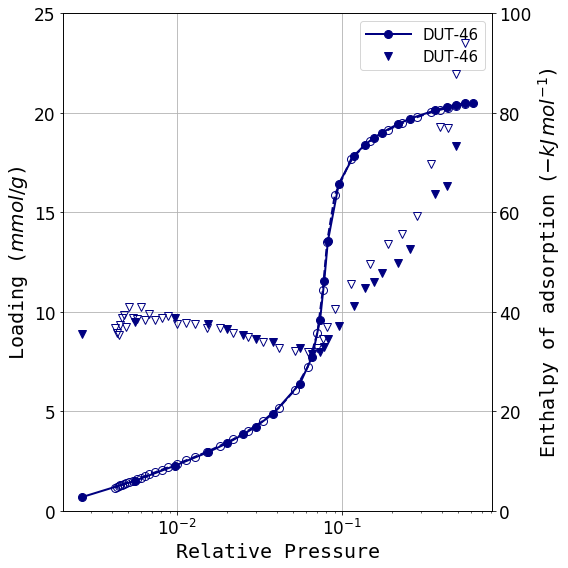
\includegraphics[width=\linewidth]{rtc/dut-46-adsdes}%
        \caption{}\label{appx:dut:fgr:dut-46-adsdes}
    \end{subfigure}%
    \begin{subfigure}{0.5\linewidth}
        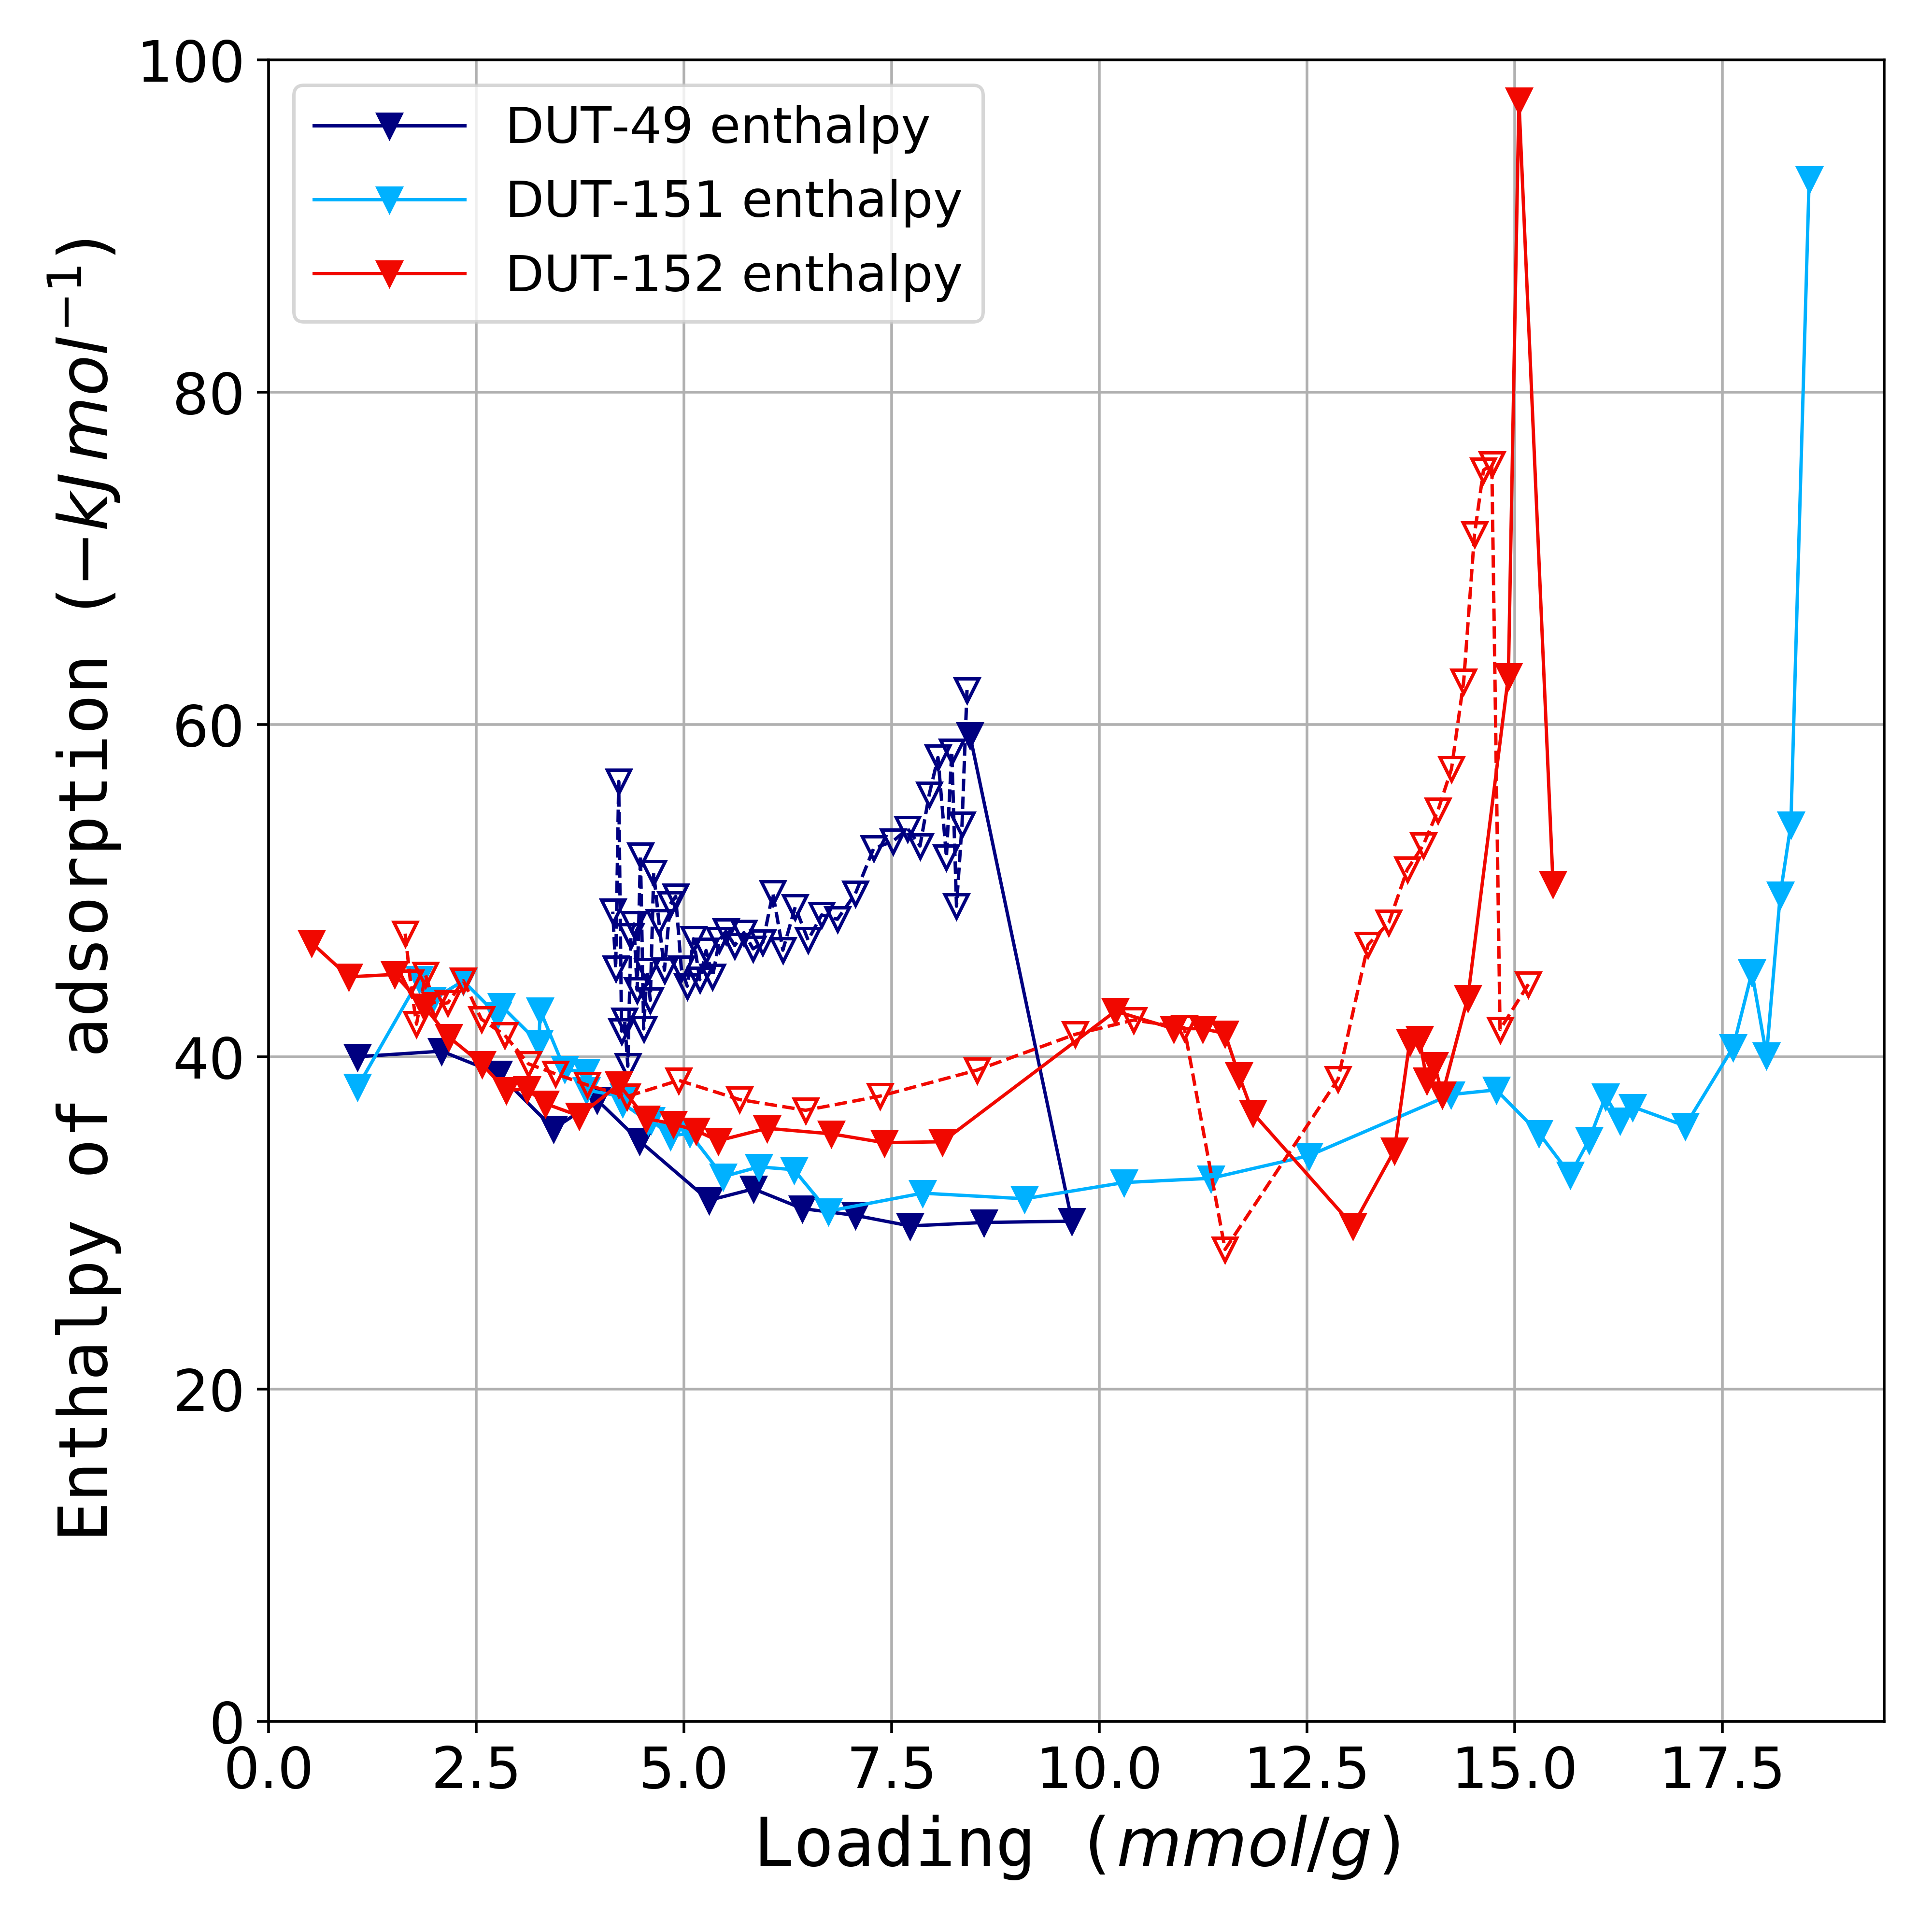
\includegraphics[width=\linewidth]{rtc/dut-reticular-interp-enth}%
        \caption{}\label{appx:dut:fgr:dut-reticular-interp-log}
    \end{subfigure}%
    \caption{The (a) isotherms and (b) enthalpy curves of the
    interpenetrated materials DUT-151 and DUT-152. Shaded regions
    are guides for the eye.}%
    \label{appx:dut:fgr:butane-extra}
\end{figure}


\bibliographystyle{unsrtnat}
\bibliography{backmatter/biblio/bib}